
\section{The \emph{Protocol Buffers} format}\label{app:protobuf_fmt}

\subsection{Introduction}

The  Google  Protocol Buffers  (\emph{protobuf})  library  is used  to
represent the objects that are exchanged between the Vire clients, the
Vire server and the CMS server.  The  version 3 of the format is used,
implying   at   least   version   3.0.0  (September   2016)   of   the
\emph{protobuf} library.

Each  data   structure  of  interest   can  be  described   through  a
\texttt{.proto}  file  from  which  stub files  can  be  automatically
generated  with the  \texttt{protoc} compiler.  For Vire  and its  CMS
interface, the C++ and Java programming languages will be used.


A  collection of  \texttt{.proto}  files are  provided  with the  Vire
library to represent all kind  of data structures transferable between
networked agents  (Vire server,  Vire clients, CMS/LAPP  server).  The
objects of  the highest level  are named \emph{payload  objects} (like
\emph{request},  \emph{response} and  \emph{event} objects).   They
are composed of attributes of more basic data structures.

\subsection{Example}

The following  class diagram  illustrates two data  structures defined
within the Vire library with an inheritance relationship between them.

\begin{center}
  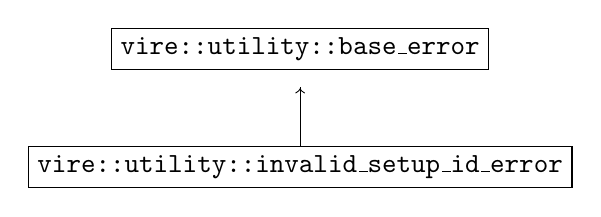
\begin{tikzpicture}
    \node (base)     at (0,1.5)  [draw] {\texttt{vire::utility::base\_error}};
    \node (setup)    at (0,0)  [draw] {\texttt{vire::utility::invalid\_setup\_id\_error}};

    \draw[->]   (node cs:name=setup,anchor=north) |- (0,1);
    |- (0,1) -| (node cs:name=base,anchor=south);
  \end{tikzpicture}
\end{center}

The \texttt{vire::utility::base\_error}  is the  parent class  for all
\emph{error}  objects.   It  contains   two  attributes:   an  integer
\emph{error code}  and a  character string describing  the \emph{error
  message}.

The   \texttt{vire::utility::invalid\_setup\_id\_error}  class   is  a
specialized error class  which represents explicitely an  error due to
an identification  failure of  the experimental setup.   It implements
additional mutually exclusive attributes: the \emph{unrecognized name}
of the setup or the \emph{unrecognized version} of the setup.

This   example  illustrates   the  protobuf   representation  of   the
\texttt{vire::utility::base\_error}  in the  Vire  library, using  the
\texttt{"vire/utility/BaseError.proto"} file:

\small
\begin{Verbatim}[frame=single,xleftmargin=0.cm,label=\fbox{protobuf}]
  syntax = "proto3";
  package vire.utility; // Namespace

  message BaseError {

    // reserved 1; // Reserved for _base message

    // Attributes:
    int32  code           = 100; // The error code
    string message_format = 101; // The error description message

  }
\end{Verbatim}
\normalsize

\vfill
\clearpage
\pagebreak

\subsection{Vire protobuf conventions}

Vire uses the following conventions:

\begin{enumerate}

\item
  The member index  \texttt{1} is reserved to represent the  link of a
  class to its main base/parent class (if any).  It is not used if the
  data structure does not inherit any data structure.
  If a data structure naturally inherits another one, it is thus possible
  to  represent the  inheritance  relationship as  illustrated with  the
  \texttt{"vire/utility/InvalidSetupIdError.proto"}      file      which
  represents the \texttt{vire::utility::invalid\_setup\_id\_error} class
  in the Vire library:

  \small
  \begin{Verbatim}[frame=single,xleftmargin=0.cm,label=\fbox{protobuf}]
    syntax = "proto3";
    package vire.utility; // Namespace

    import "vire/utility/BaseError.proto"; // Dependency

    message InvalidSetupIdError {

      BaseError _base = 1; // The base class

      // Additional attributes:
      oneof detail { // Mutual exclusion
        string invalid_setup_name    = 100; // The failed setup name
        string invalid_setup_version = 101; // The failed setup version
      }

    }
  \end{Verbatim}
  \normalsize

\item The  \texttt{\_base} member  is conventionally  used to  represent the
  inheritance   relationship    from   a   data   structure    of   type
  \texttt{"vire.utility.BaseError"}.

\item Member indexes from \texttt{2}  to \texttt{99} are also reserved
  for possible future usage (multiple inheritance, metadata\dots).

\item
  The first member of the data structure must start at index \texttt{100}.

\end{enumerate}

\vfill
\clearpage
\pagebreak

% end
